% !TeX root = ../main.tex

\chapter{Results}\label{results}
\section{Outcomes of Interest}
Although we can construct the mobile communication network features based on two directions of mobile communication---incoming and outgoing---we will focus on the outgoing direction as the variation in outgoing-based features may be more sensitive to the factors directly linked to the treated units themselves.
Moreover, through observing Figures in \nameref{appendix_event_centered_trends}, where various outcomes' paths during the whole sample period are plotted, we can see that the evolution patterns typically don't have dramatical differences between outgoing and incoming communication.
Therefore, when discussing the treatment effects of both residential shift and smartphone adoption, we will consider only the outgoing-based mobile communication features.
For mobility features, although we propose a new weighting scheme to address the issue of spurious importance of telecom base stations for phone users, arising from the routing mechanism, it seems that mobility features' differences between two construction methods based on distinct weighting schemes are subtle (see \nameref{appendix_event_centered_trends}).
Hence, we will adopt our proposed weighting scheme based on the concept of temporal size to compute the mobility features.
All in all, outcomes consists of two groups: mobility features and mobile communication network features, and there are three outcomes in each group.
The total of six outcomes focuses on capturing different aspects of human's mobility and mobile communication behavior.

\section{Selection of Anticipation Parameter}
In this section, we explain how we determine the anticipation parameter $\delta$, which is the number of months allowed for anticipation.
As we aim to identify effects of residential shift and smartphone adoption on two groups of outcomes---mobility and mobile communication network features---it is plausible for migrants to change their mobility and mobile communication behavior prior to their relocations, as explained previously.
However, it's subtle whether users will anticipate upgrading their devices to smartphones.
Therefore, we will primarily focus on the residential shift as an illustration example and apply the strategy developed in this section on both treatment contexts.

To select the correct horizon of $\delta$, we initiate a warm-up estimation for the group-time ATT by applying the \cite{callaway2021difference}'s method implemented in the \textit{did} R package.\footnote{The \textit{did} R package, to which both authors of the paper, \cite{callaway2021difference}, have been contributing.}
Several critical settings include setting the \textit{anticipation} argument to 0, corresponding to $\delta = 0$ and the \textit{base\_period} argument to ``varying''. Moreover, we rely on the conditional parallel trend assumption and the never-treated control units.
By setting the \textit{anticipation} argument to 0, the post-treatment estimation on group-time ATT is referred to the one period (month) prior to residential shift, and the ``varying'' \textit{base\_period} allows the group-time ATT to be estimated in the reference period, unlike the conventional event study design\footnote{The \textit{did} R package allows the event study design by setting \textit{base\_period} to ``universal''.}.

In traditional event study, outcomes in both post-treatment and pre-treatment periods are compared to the reference period, which is the one period prior to the treatment if there is no anticipation.
Therefore, the reference period cannot compare to itself, resulting in the failure of estimation.
Nonetheless, ``varying'' \textit{base\_period} means that for each period before the treatment, the group-time ATT is estimated through iteratively changing the reference period.
That is, to estimate the ATT in one month prior to the treatment, which is usually the reference period, the two periods prior is employed as reference.

``Varying'' \textit{base\_period} is plausible in pre-treatment periods as it relies on the PTA specific to two-period DiD (see Equation \ref{eq:parallel_trend}), which involves the short difference, i.e., $Y_{i, m} - Y_{i, m-1}$, instead of the long difference $Y_{i, m} - Y_{i, g-\delta-1}$ utilized in the post-treatment estimation of DiD with multiple periods (see Equation \ref{eq:parallel_trend_general_first}) within each treatment group's estimation of ATT dynamics.
The motivation for the long difference is that \( Y_{i, m-1}(\infty) \) is still unobservable in post-treatment periods if \( m-1 \neq n-\delta-1 \) whereas this does not hold in the pre-treatment periods.
Therefore, the short difference is sufficed and applied.

The reason why we specifically want the group-time ATT to be estimable in the reference period \( g-\delta-1 \)	 is that it is the most likely period for treatment cohorts to anticipate.
Furthermore, iteratively changing the reference period allows us to more easily observe the jump in the plot of group-time ATT dynamics during the pre-treatment period, thereby hypothesizing the occurrence of the anticipation behavior.
Moreover, It's relatively computationally efficient compared to conventional event study in that we only need one estimation procedure by setting \textit{base\_period} to ``varying'' to have complete ATT estimation in all pre-treatment periods.
Nevertheless, since event study can't estimate ATT in the reference period, we may need to try out different anticipation values, running several estimation procedures to find the right one.

One can view the estimation of ATT in the pre-treatment periods as the placebo test, which aims to answer a hypothetical question: what is the treatment effects if the users pretendedly receive the treatment prior to the real treatment timing?
If the treatment is not confounded, anticipation parameter $\delta$ is correctly specified, and PTA holds, the placebo test should yield an insignificant ATT.

\begin{figure}[h!]
\centering
\caption{Aggregate Event Study of Residential Shifts with No Anticipation}
\vspace{0.1cm}

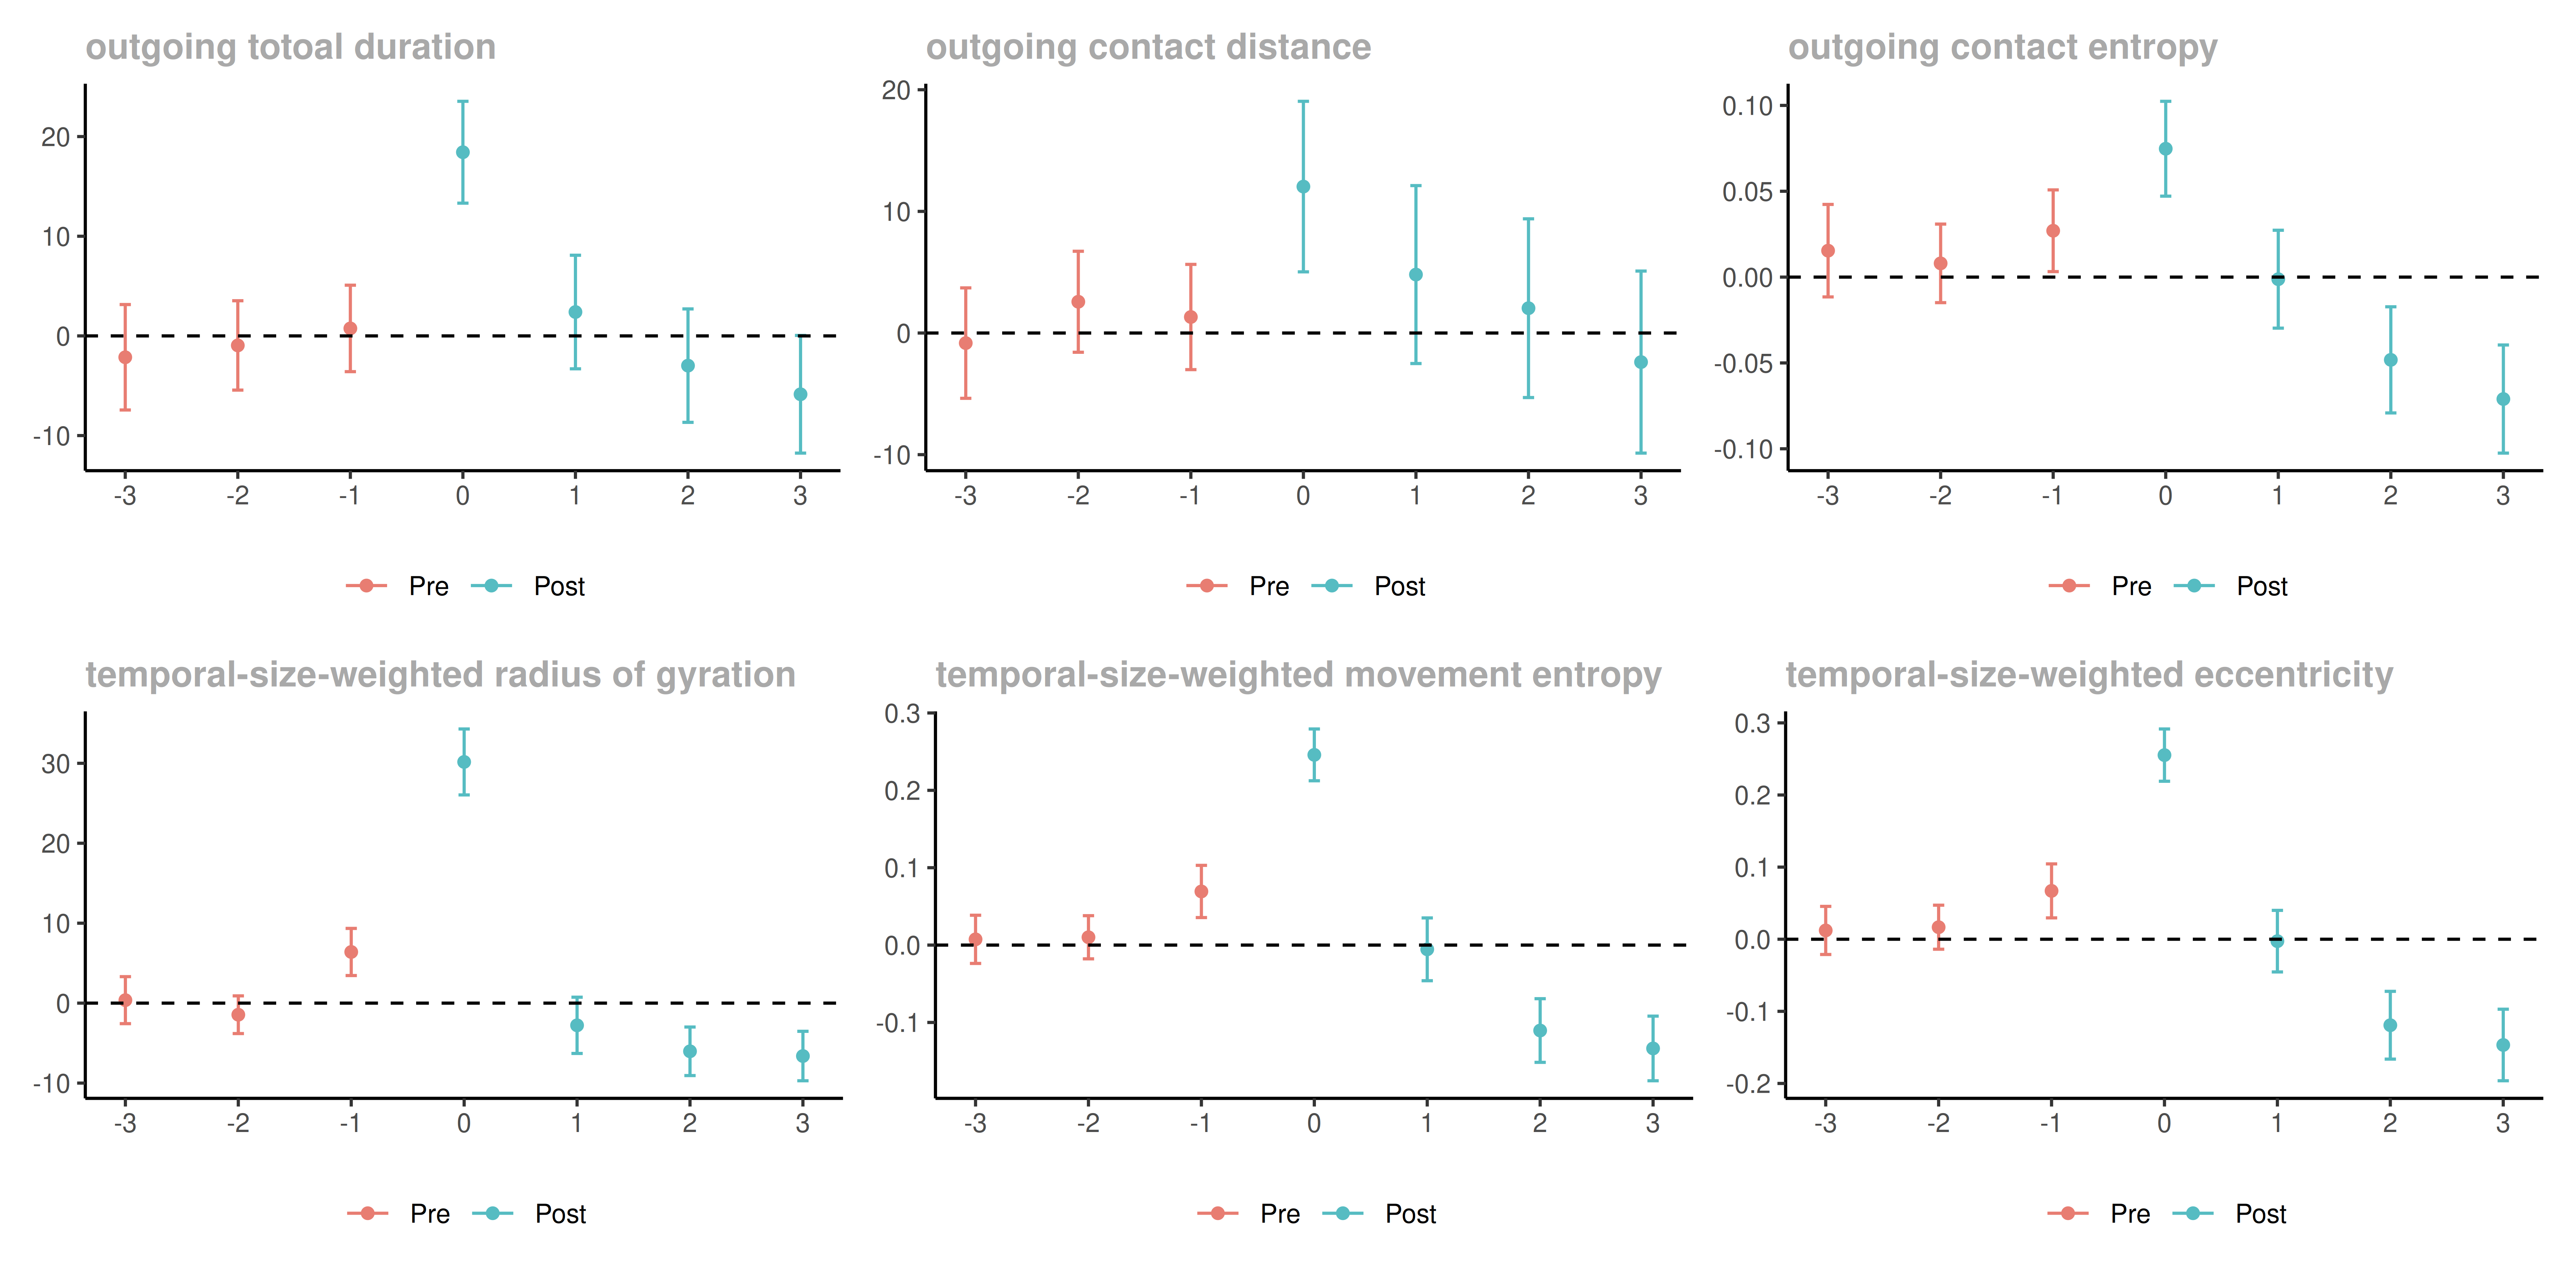
\includegraphics[width=1\textwidth]{figures/csdid/inspect_delta/residential_shift.png}

% \caption*{Note the x-axis is the month relative to the treatment timing.}
\label{fig:select_delta_residential_shift}
\end{figure}

In Figures~\ref{fig:select_delta_residential_shift}, we plot the warmup estimation results of group-time ATT of residential shift on two groups of features.
We can see that the group-time ATT is very often significantly different from 0 in the one-month prior to the residential shift and the ATT in period \( g-1 \) (event time -1) is in the same direction with the period \( g \) (event time 0).
Note that we employ the 95\% confidence bands.
Therefore, we think that the number of months for anticipation \( \delta \)	 should be set to one when discussing treatment effects of residential shift.
% It is interesting to see that in mobility patterns, the anticipation seems to be involved in all three different features, while in mobile communication network features, the anticipation seems to emerge more often in the incoming direction, which potentially indicates the unique characteristics of long-distance contacts in the mobile communication network. For instance, as relocation information spreads through local neighbor networks, distant friends may respond with increased incoming calls to show support, while local contacts can express concern through direct meetings. On the other hand,

Note that for some outcomes, such as outgoing duration and contact distance, it doesn't make sense to claim the existence of anticipation as ATT in event time -1 (period \( g-1 \)	) denoted as \( ATT(-1) \) is insignificant.
However, it won't affect the estimation of post-treatment effect on these outcomes when requiring the anticipation months to be one, i.e., \( g-2 \) is referenced.
This is because as the ``varying'' \textit{base\_period} let $ATT(-1)$ be obtained by referencing period $g-2$, and as the plot shows, $ATT(-1)$ is insignificant, which means the difference, $\mathbb{E}[Y_{i, g-1} - Y_{i, g-2} \mid G_{i, g} = 1]$ is equivalent to the parallel trend. Therefore, it will be differenced out by $\mathbb{E}[Y_{i, g-1} - Y_{i, g-2} \mid G_{i, \infty} = 1]$.

Nevertheless, the situation is not symmetric for outcomes other than outgoing duration and contact distance when we incorrectly set \( \delta = 0 \) while the true value is \( \delta = 1 \).
This asymmetry arises because \( Y_{i,g-1} \) contains an ATT component, and differencing other periods' outcomes against this contaminated baseline distorts the ATT estimates in those periods.
Specifically, the ATT in other periods will be underestimated when treatment effects across periods have the same sign, but amplified when they have opposite signs.

Regarding the treatment of smartphone adoption, it seems to be unfair to claim the existence of anticipation, and through the plot, we don't find the evidence of pre-treatment shifts in outcomes, therefore we will set $\delta$ to 0.

\begin{figure}[h!]
\centering
\caption{Aggregate Event Study of Smartphone Adoption with No Anticipation}
\vspace{0.1cm}

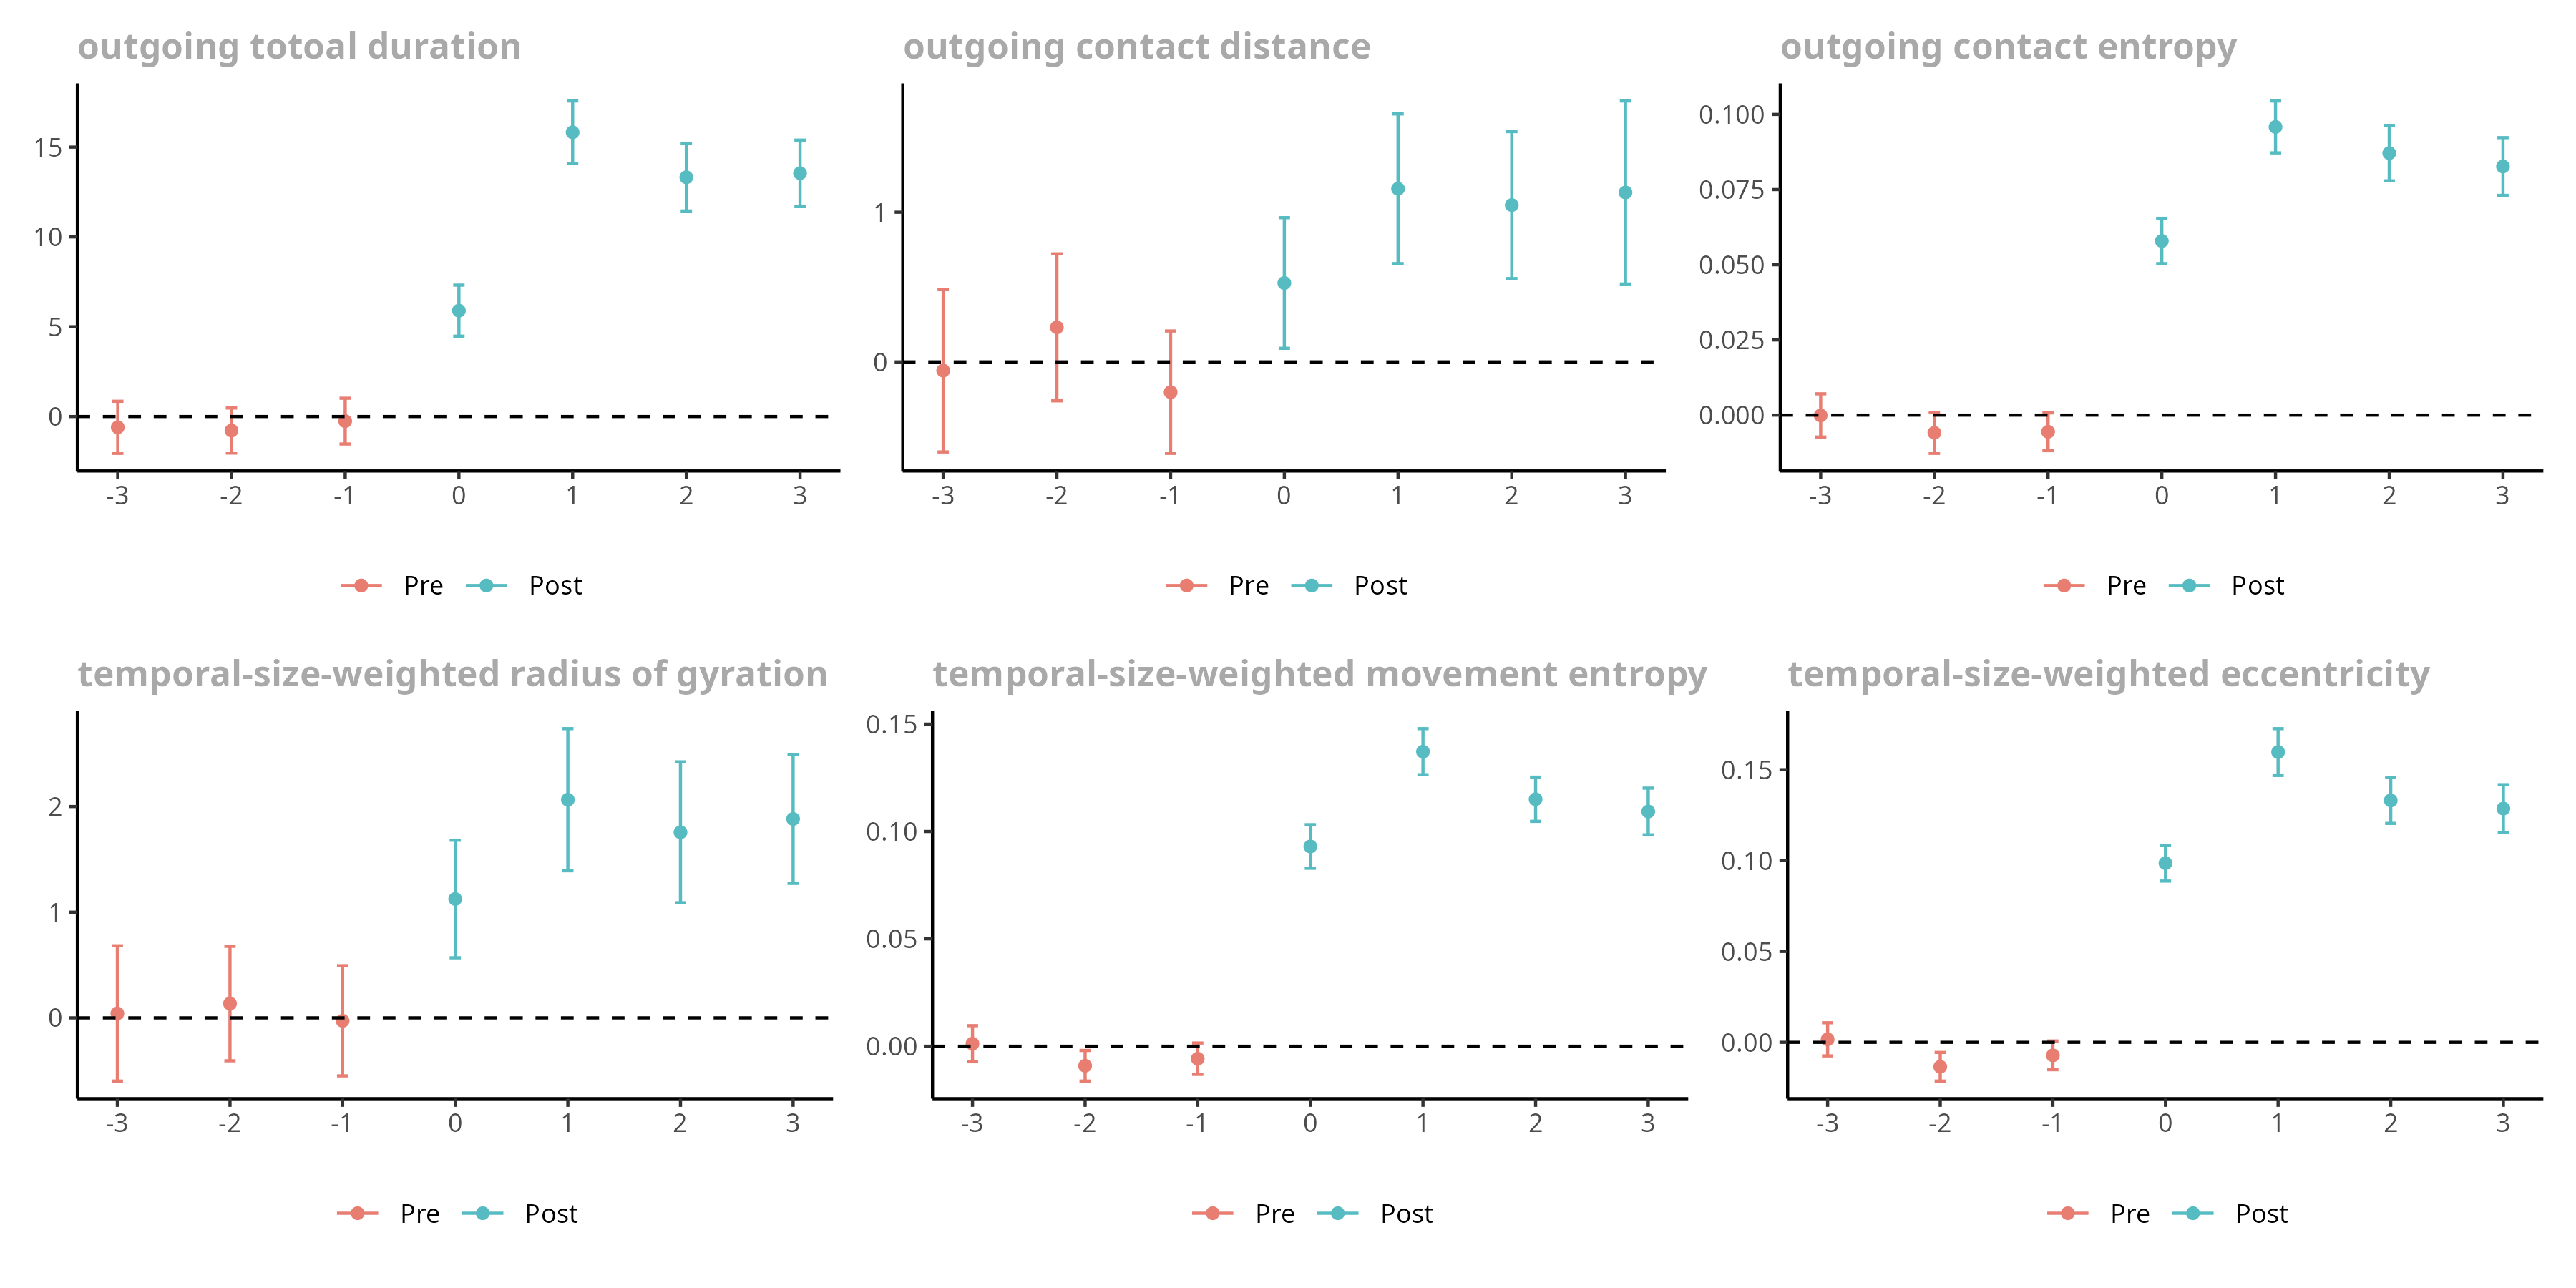
\includegraphics[width=1\textwidth]{figures/csdid/inspect_delta/smartphone_adoption.png}

% \caption*{Notes: }
\label{fig:select_delta_smartphone_adoption}
\end{figure}

\clearpage\newpage
\section{Residential Shift}\label{main_res_residential_shift}
In the current and next section, we are going to analyze the estimation restuls of ATT with the delicately determined \( \delta \), ``universal'' \textit{base\_period}, and the assumption of unconditional PTA. The confidence interval is constructed based on the 95\% significance level. We first analyze heterogeneous treatment effects across time periods. Specifically, we will approach with a hierarchical manner starting from the discussion of static versus time-variant treatment effects. The static treatment effect means the outcome is persistently shifted without fading back to the baseline level. In such situation, attribution includes upward or downward shift. For the time-variant one, we can characterize it to be either transient or smoothly decaying. A transient treatment effect over time represents an effect that instantly bounces back and forth to the baseline, while smoothly decaying is the other case, where the effect gradually fades away. Then, we can discuss the heterogeneous effect across treatment-timing groups by inspecting whether only few groups exhibit distinct patterns.


\begin{figure}[h!]
\centering
\caption{Aggregated Event Study of Residential Shifts}
\vspace{0.1cm}

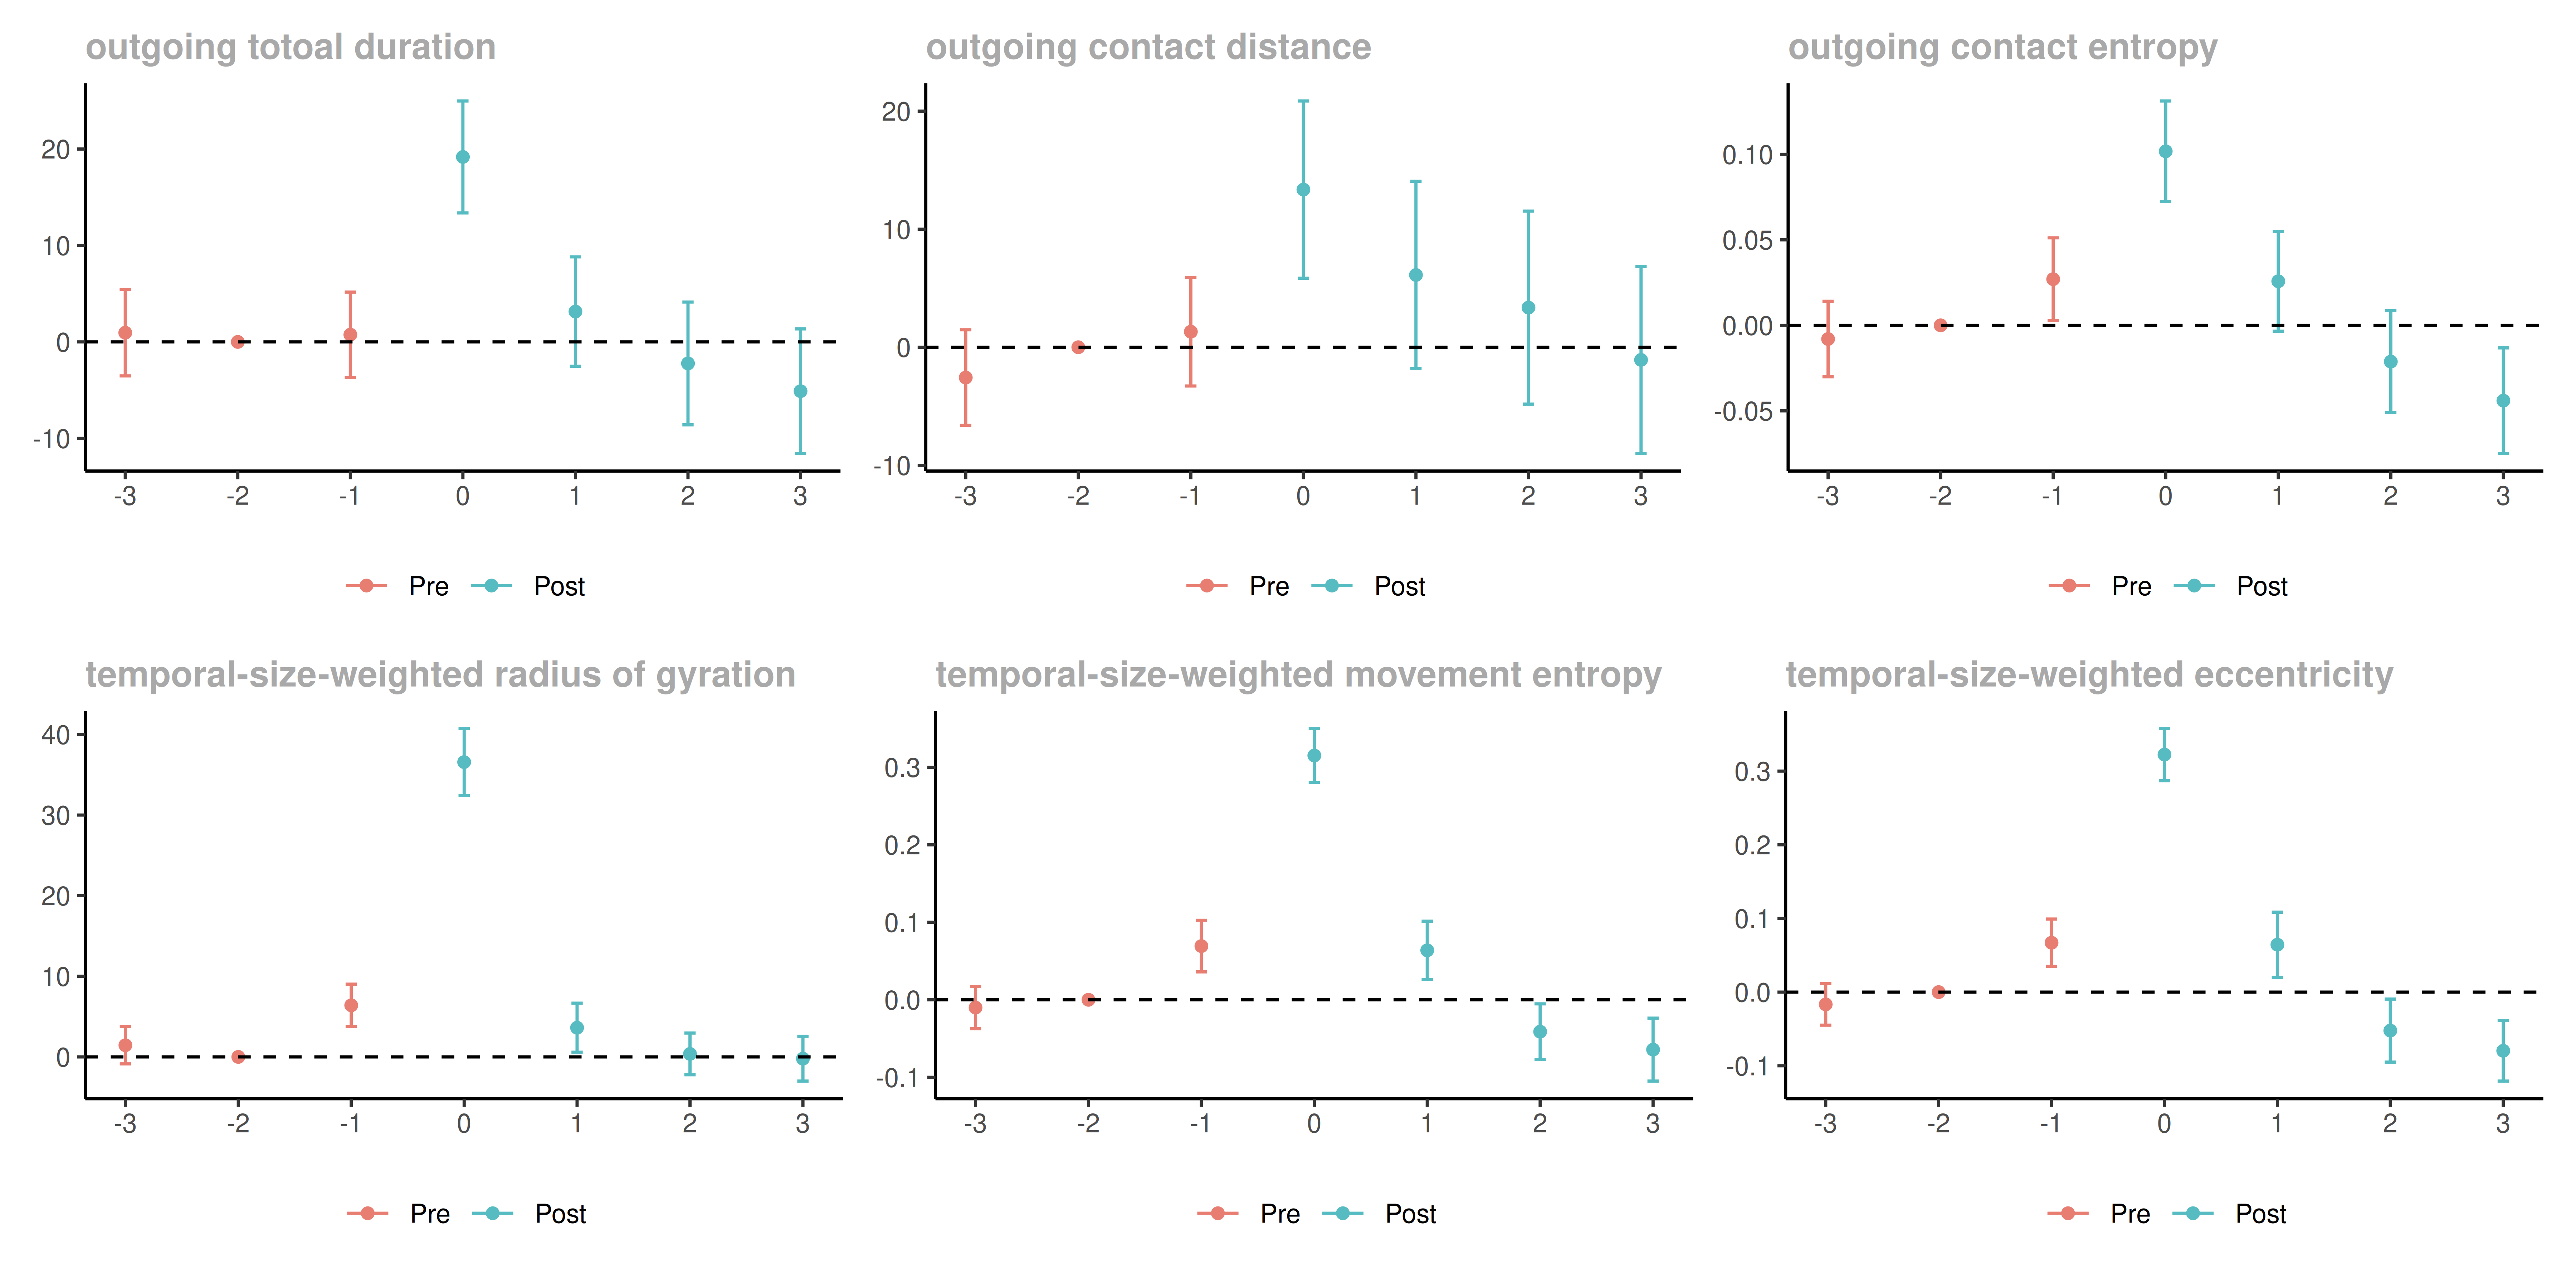
\includegraphics[scale=0.49]{figures/csdid/residential_shift.png}

% \caption*{Notes:}
\label{fig:event_study_residential_shift}
\end{figure}

At the very first glance, we can see that the residential shift brings about time-variant effects on both mobile communication network (upper panel) and mobility features (lower panel), and effects fall back to or approach to the baseline level one month after relocations begin.

For the mobile communication behavior, anticipation for residential relocation is limited and observable only in outgoing contact entropy.
The pre-treatment shift in outgoing contact entropy might be result from notifying forthcoming relocation with friends that are less frequently contacted.
However, from Figure \ref{fig:attgt_residential_shift_mobile_communication_network}, we can see that this phenomenon only emerges in the treated units who migrate in February 2014 (group 7).

Intuitively, residential relocations expose mobile phone users to unfamiliar environments, resulting in a temporary surge in total call duration during the month of relocation with increases of 19 minutes in outgoing call duration and 13 km in outgoing contact distance as migrants may seek to contact with geographically distant social connections.
Moreover, during this same period, migrants engage in more diversified social interactions, likely due to the formation of new social connections at the destination or contact with those with whom they engaged less frequently prior to the relocation.
Nevertheless, following the completion of relocation, migrants tend to spend less time on mobile communication with less diversified interactions. Moreover, the decreasing outgoing contact distance may be due to the composite effects of attenuated formal friendships and new local connections around the neighborhood of destination.


\clearpage\newpage
\begin{figure}[h!]
\centering
\caption{Contact Ratio of Pre-Treatment Friends in Post-Treatment Periods}

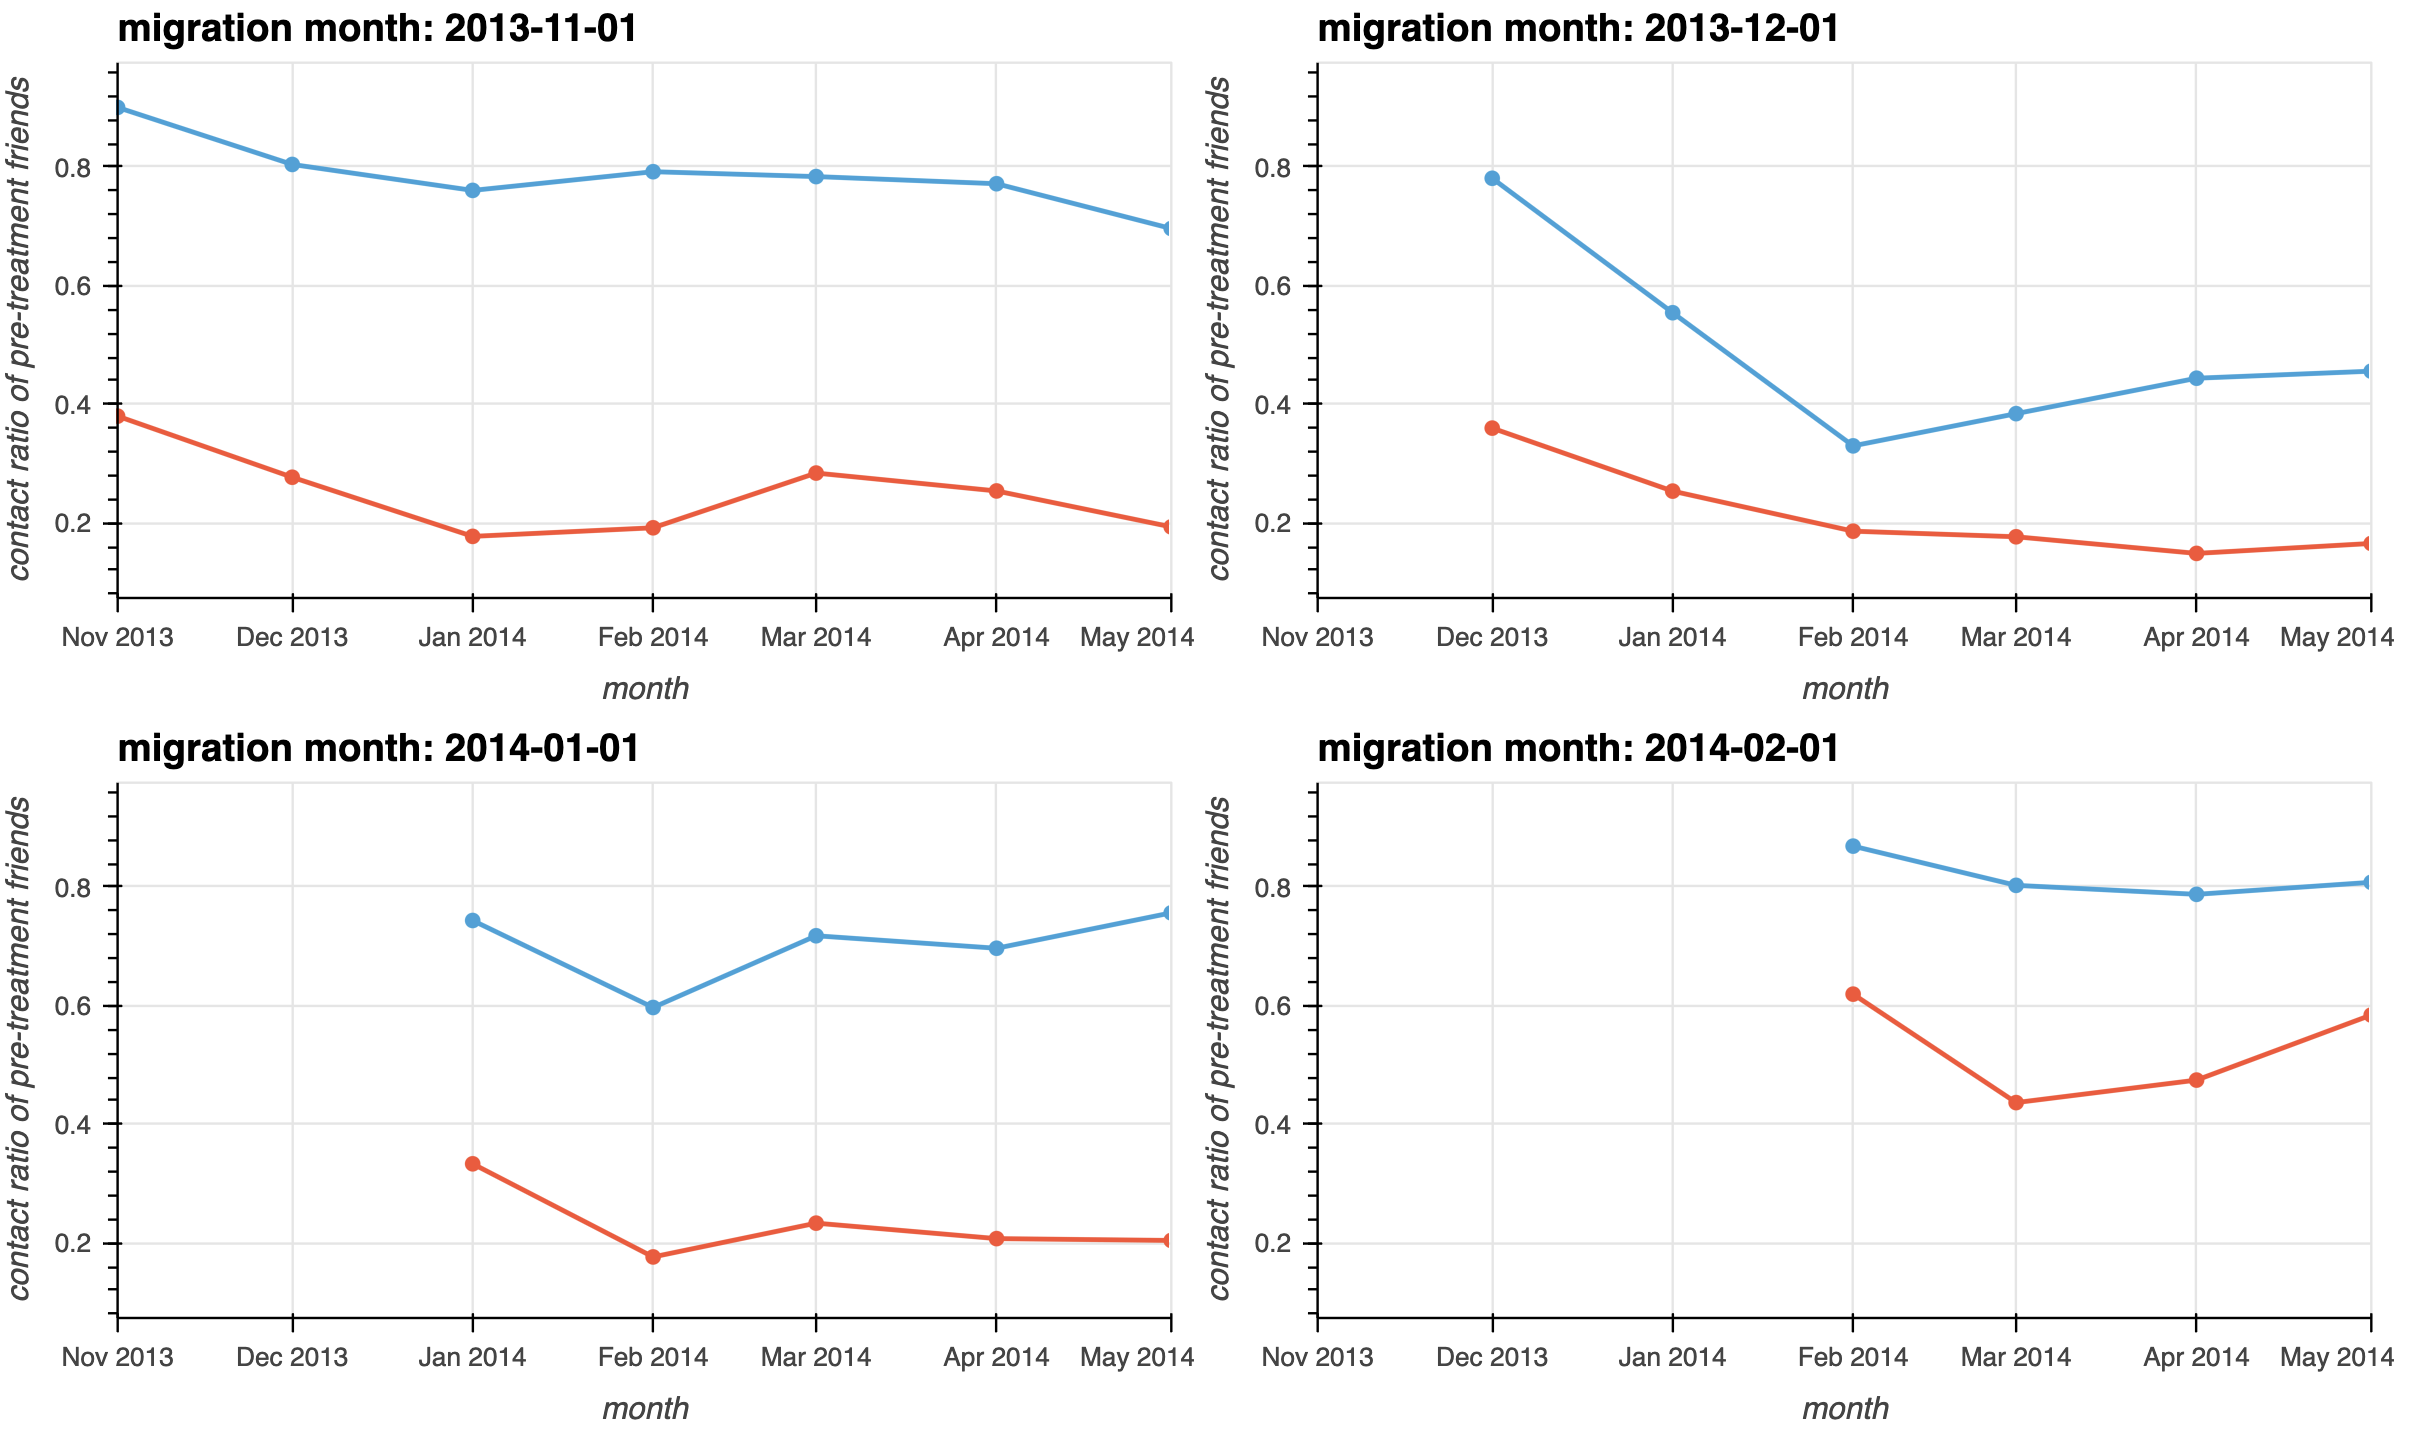
\includegraphics[scale=0.35]{figures/contact_ratio_of_pretreatment_friends.png}

\caption*{Notes: The blue line is the contact ratio of pre-treatment friends while the red line additionally require those in the same origin prefecture.}
\label{fig:contact_ratio_old_friends}
\end{figure}


In Figure \ref{fig:contact_ratio_old_friends}, we analyze the composition of migrants' contacts in post relocation periods.
We define a new variable called contact ratio, and the contact ratio of a user in a given month measures the proportion of the users' call duration with friends with whom they are already connected versus all friends contacted in the corresponding month.
In the above plot, we present the monthly contact ratio series obtained by averaging across all users in each given month.
We also separately plot the contact ratios for migrants who relocate in different months though they seem to behave very similarly.

We can confirm that, in the early periods of post-migration, migrants tend to connect with those old friends with whom are already connected prior to the migration events.
Typically, in the same months of changing residential places, around 80\% of contacts are pre-treatment friends, but they are not necessarily in the same prefectures from which migrants come.
Specifically, roughly 40\% of these pre-treatment friends reside in the migrants' origin prefecture.
These facts support the hypothesis that the sudden surge in mobile communication during the period of migration is due to connections with existing friendships.
Moreover, the drastic increase in contact distance also suggests that migrants move away from their friends rather than toward them.

For mobility patterns, the evidence of anticipation behavior is even more solidified, with moderate upward shift. The spatial coverage of movement activity measured through the metric of radius of gyration substantially increases contemporaneously with the completion of residential relocation, increasing by 36.6 km while the effect quickly fades back in the following months. Movement entropy and eccentricity evolve in an extreme pattern where migrants instantly transit from highly unpredictable spatial appearances with spatial stretching along a fixed direction to predictable patterns with roughly circular or round spatial distribution, characterized by a dramatic shift from +0.32 above baseline for both entropy and eccentricity to -0.06 and -0.08 below baseline respectively. The intuition is when moving to a new environment, a migrant might be actively exploring but have limited knowledge, resulting in exploring along with a fixed axis. As time goes by, the exploration patterns settle down, and they might only mainly visit a few places located on various directions.

In conclusion, residential shifts produce distinct anticipation effects between communication and mobility domains, with mobility patterns showing more pronounced responses than communication behaviors. Moreover, both groups of features seem to be continuously evolving to negative states. To better understand the evolving paths of various features across treatment-timing groups, please refer to \nameref{complete_group_time_att_dynamics}.

\clearpage\newpage
\section{Smartphone Adoption}
\begin{figure}[h!]
\centering
\caption{Aggregate Event Study of Smartphone Adoption}
\vspace{0.1cm}

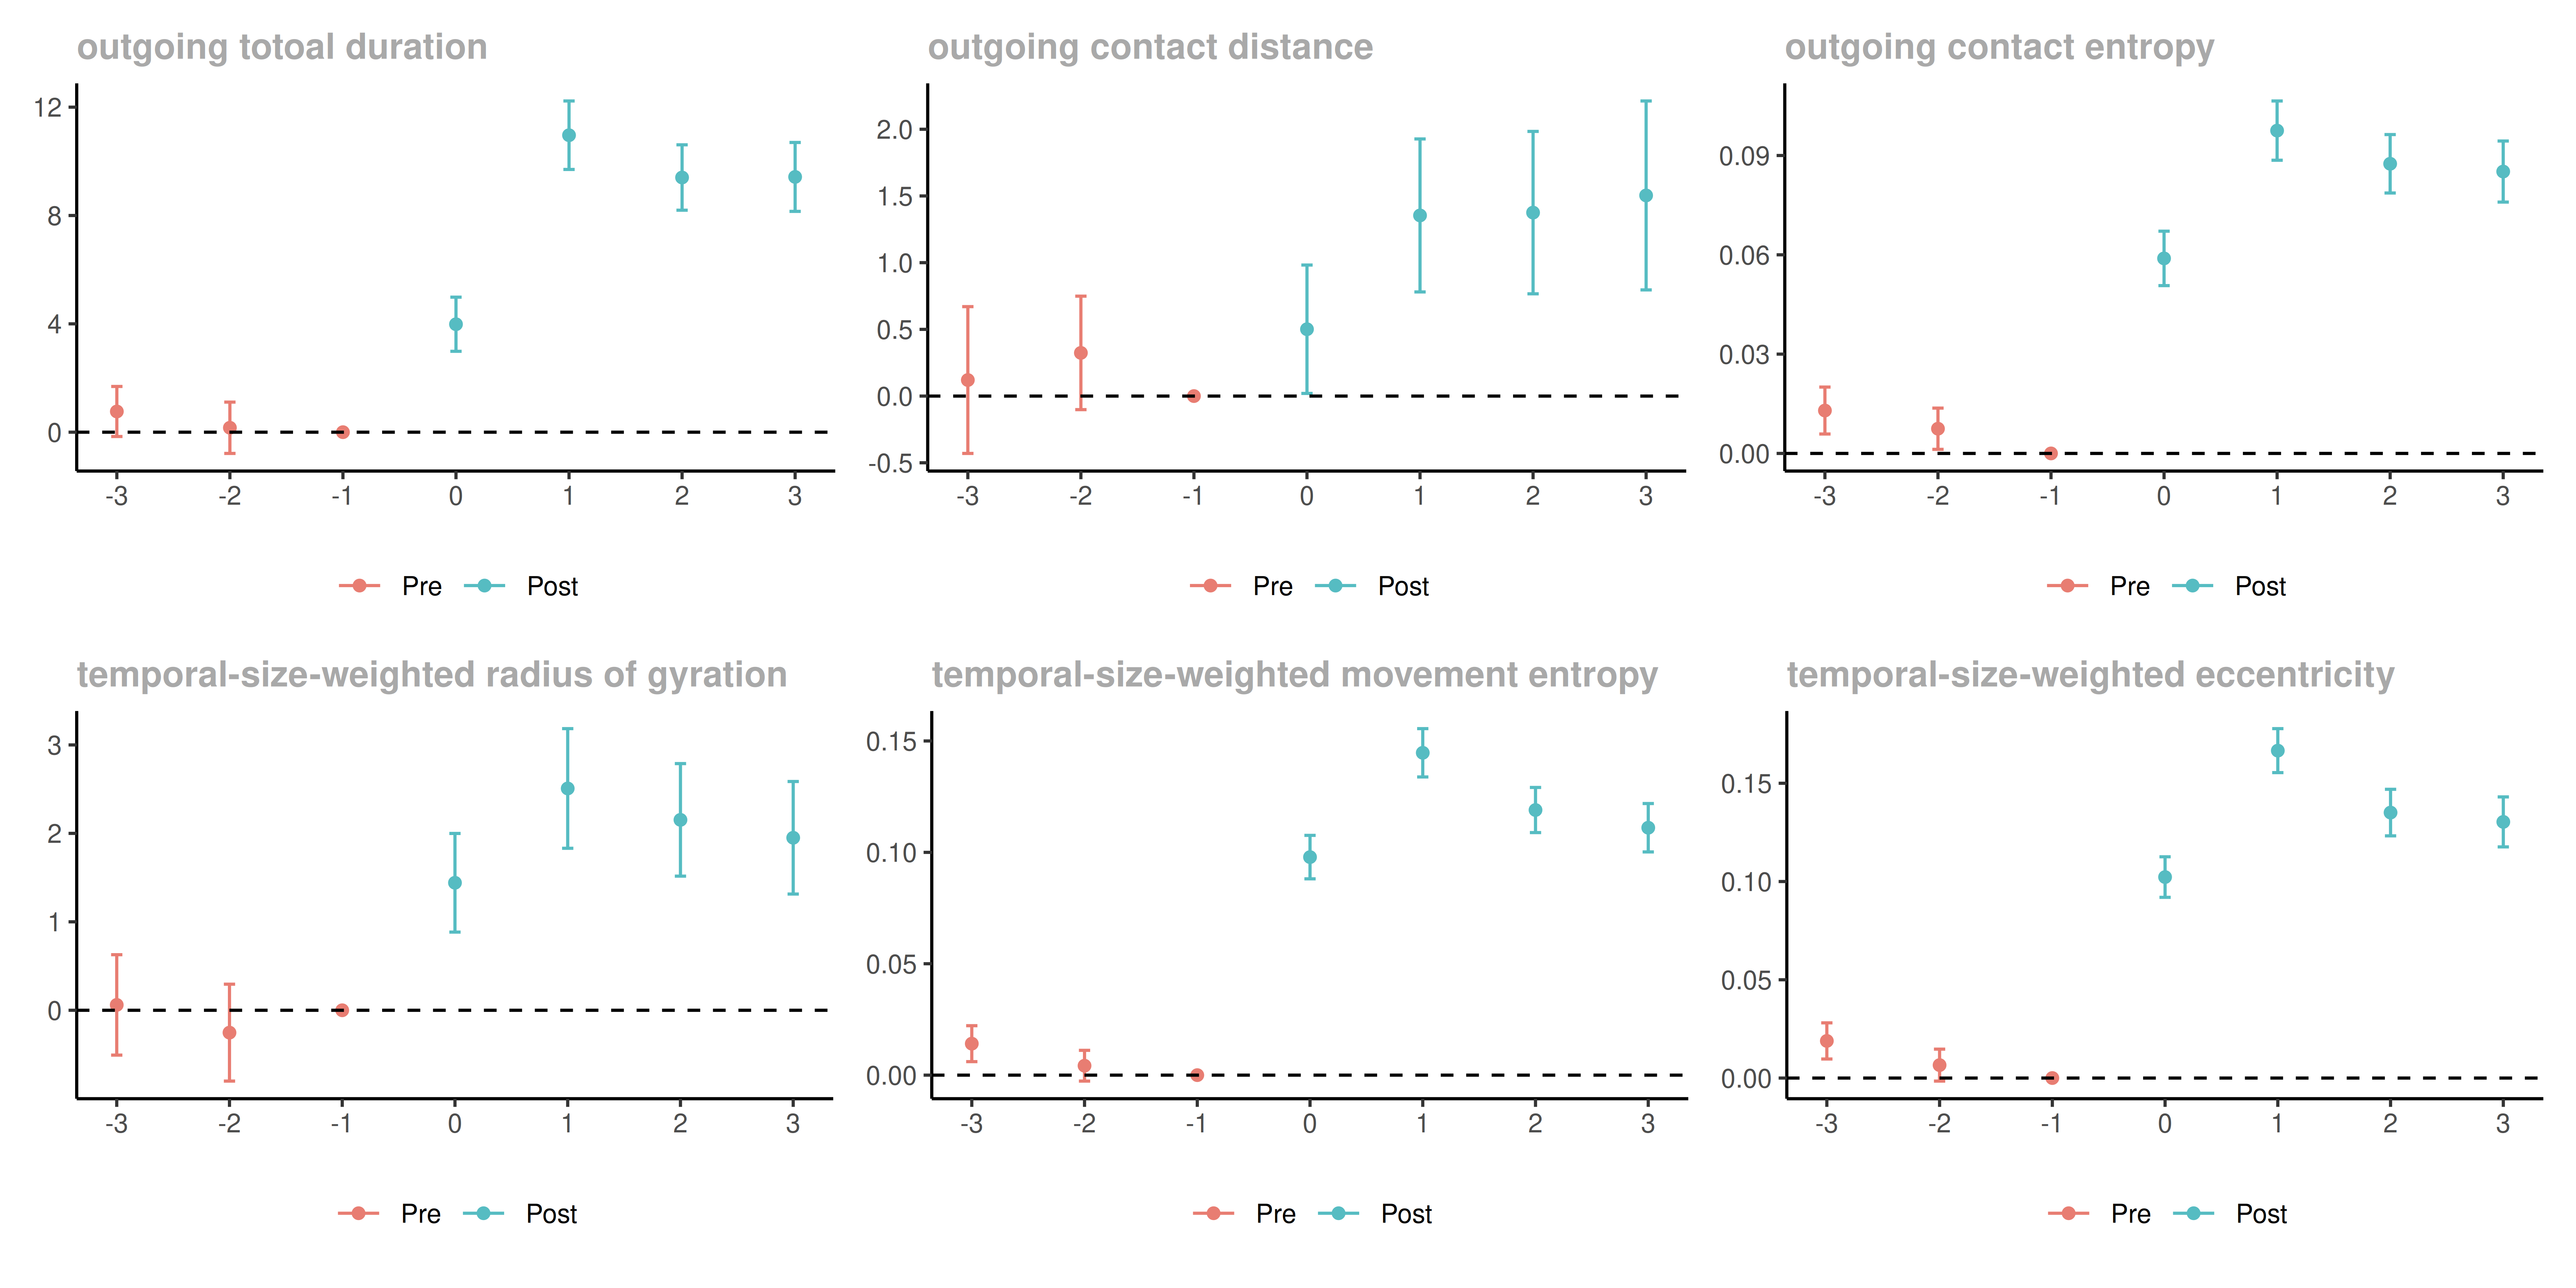
\includegraphics[scale=0.49]{figures/csdid/smartphone_adoption.png}

% \caption*{Notes:}
\label{fig:event_study_smartphone_adoption}
\end{figure}

Unlike the residential shift, we expect no anticipation for smartphone adoption.
We clearly see that the effects are nearly static over time and the shifts are positive, but the magnitude is relatively small compared to the residential shift.
By inspecting ATT dynamics across different groups demonstrated in both Figure \ref{fig:attgt_smartphone_adoption_mobile_communication_network} and \ref{fig:attgt_smartphone_adoption_mobility}, we can confirm that there is no heterogeneous effect across groups.
The most notable influence is the increase in outgoing total call duration with a magnitude of 17 minutes in the first month after switching devices to smartphones.
Besides, the modest upward shifts in both movement entropy and eccentricity might be due to the integration of geographical technologies, such as online maps, facilitating the exploration of unfamiliar places.
Therefore, individuals' movement trajectories become more unpredictable and their visited places become richer in the directional sense, leading to more spatially distributed mobility patterns.
